\documentclass{article}

\usepackage[margin=1in]{geometry}
\usepackage{amsmath,amsthm,amssymb}
\usepackage{bbm,enumerate,mathtools}
\usepackage[hidelinks]{hyperref}
\usepackage{tikz}
\usetikzlibrary{matrix, arrows}

\newenvironment{problem}[2][Problem]{\begin{trivlist}
\item[\hskip \labelsep {\bfseries #1}\hskip \labelsep {\bfseries #2.}]}{\end{trivlist}}
\newenvironment{note}[1][Note.]{\begin{trivlist}
\item[\hskip \labelsep {\bfseries #1}]}{\end{trivlist}}
\newenvironment{problempart}[1]{\begin{trivlist}\item[\textbf{Part #1.}]}{\end{trivlist}}


\begin{document}

\title{Differential Geometry: Homework 6}
\author{Peter Kagey}

\maketitle

% -----------------------------------------------------
% First problem
% -----------------------------------------------------
\begin{problem}{1} \text{} \\
  \begin{enumerate}[(a)]
    \item  Write in detail the construction of the canonical map
      $V^* \otimes W \xrightarrow{\alpha} \hom(V, W)$,
      and give a careful proof that it is an isomorphism if $V$ and $W$ are
      finite dimensional.
    \item Let $ev\colon V^* \otimes V \rightarrow \mathbb{R}$ be the linear map
    induced by the bilinear map
    $\overline{ev}\colon V^* \times V \rightarrow \mathbb{R}$,
    $(\phi, v) \mapsto \phi(v)$ by the universal property of the tensor product.
    Given a linear operator $T \in \hom(V, V)$ on a finite dimensional vector
    space define \[
      tr(T) := ev(\alpha^{-1}(T)).
    \]

    Show that this definition agrees with the usual definition of trace.
  \end{enumerate}
\end{problem}

\begin{proof} \text{} \\
  \begin{enumerate}[(a)]
    \item Firstly there exists a bilinear map
    $\eta\colon V^* \times W \rightarrow \hom_\mathbb{R}(V, W)$ given by \[
      (v^*, \vec{w}) \mapsto
        (\vec{v} \mapsto \underbrace{v^*(\vec{v})}_{\in \mathbb{R}}\vec{w}).
    \] Because $\hom(V, W)$ is an $\mathbb{R}$-vector space, by the universal
    property, there exists a unique linear map $\alpha = \bar{\eta}$ such that
    the diagram \[
      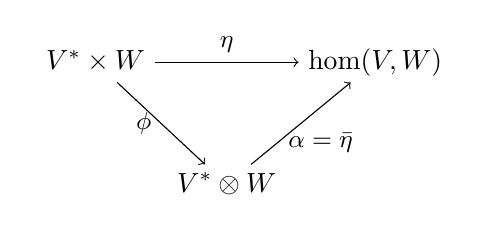
\begin{tikzpicture}[description/.style={fill=white,inner sep=2pt}]
        \matrix (m) [matrix of math nodes, row sep=3em,
        column sep=0.5em, text height=1.5ex, text depth=0.25ex] {
          V^*\times W & & \hom(V, W) \\
          & V^* \otimes W & \\
        };
        \path[-,font=\small]
          (m-1-1) edge[->] node[auto] {$\eta$} (m-1-3)
          (m-1-1) edge[->] node[left] {$\phi$} (m-2-2)
          (m-2-2) edge[->] node[below] {$\hspace{0.5cm}\alpha = \bar{\eta}$} (m-1-3);
      \end{tikzpicture}
    \] commutes.
    Because the universal property gives that $\alpha$ is a linear map, it is
    sufficient to check that $\alpha$ has a two-sided inverse.
    Let $\underline{v} = (v_1, \hdots, v_k)$ and
    $\underline{w} = (w_1, \hdots, w_r)$ be bases for $V$ and $W$ respectively,
    and let $\underline{v}^* = (v^*_1, \hdots, v^*_k)$ be the associated dual
    basis for $V^*$. Then $\{v_i^* \otimes w_j\}_{(j, i)}^{(k, r)}$ is a basis
    for $V^* \otimes W$, and $\{v_i^*(-)w_j\}_{(j, i)}^{(k, r)}$ is a basis for
    $\hom(V, W)$.

    Then $\alpha^{-1}$ is the map that sends
    $v_i^*(-)w_j \mapsto v_i^* \otimes w_j$, extended by linearity, and thus
    $\alpha$ is an isomorphism.
    \item
    Let $\psi\colon V^* \times V \rightarrow V^* \otimes V$ map
    $(\phi, v) \mapsto \phi \otimes v$. Then by the universal property of
    tensor products,
    $\overline{ev} = ev \circ \psi$. That is, $ev$ maps
    $\phi \otimes v \mapsto \phi(v)$.

    Let $\underline{v} = (v_1, \hdots, v_n)$ be a basis for $V$ and
    $\underline{v}^* = (v^*_1, \hdots, v^*_n)$ be the associated basis for $V^*$
    as above.
    Then \begin{align*}
      T(\vec{v}) &= \sum_{j=1}^n v^*_j(\vec{v})T(v_j) \\
      &= \sum_{j=1}^n v^*_j(\vec{v})\left(
        \sum_{i=1}^n A_{ij}v_i
      \right)\\
      &= \sum_{i,j=1}^n A_{ij} v_j^*(\vec{v})v_i
    \end{align*}
    Applying $a^{-1}$ yields \[
      a^{-1}(T) = \sum_{i,j=1}^n A_{ij} v_j^* \otimes v_i,
    \] and further applying $ev$ gives \begin{align*}
      ev(a^{-1}(T))
        &= \sum_{i,j=1}^n A_{ij} v_j^*(v_i)\\
        &= \sum_{i,j=1}^n A_{ij} \delta_{ij}\\
        &= \sum_i^n A_{ii}\\
        &= tr(A)
    \end{align*} where $v_i^*(v_j) = \delta_{ij}$, the Kronecker delta, by
    construction of the associated dual basis for $V^*$.
  \end{enumerate}
\end{proof}

% -----------------------------------------------------
% Second problem
% -----------------------------------------------------
\pagebreak

\begin{problem}{2} \textbf{Exterior algebra 1.}\\
  Suppose that $\dim V = 3$ and $\underline{v} = (v_1, v_2, v_3)$ is a
  basis for $V$. Let $T\colon V \rightarrow V$ be the linear operator
  defined by \begin{align*}
    T(v_1) &= av_1 + dv_2 + gv_3\\
    T(v_2) &= bv_1 + ev_2 + hv_3\\
    T(v_3) &= cv_1 + fv_2 + iv_3.
  \end{align*}
  Derive a formula for $\det(T)$ in terms of $a,b,c,d,e,f,g,h,$ and $i$.
\end{problem}

\begin{proof} $ $\\
  Let $\vec{w} = v_1 \wedge v_2 \wedge v_3$. Then \begin{align*}
    T(\vec{w}) &= (av_1 + dv_2 + gv_3) \wedge (bv_1 + ev_2 + hv_3) \wedge (cv_1 + fv_2 + iv_3) \\
      &= (av_1 \wedge (bv_1 + ev_2 + hv_3) + dv_2 \wedge (bv_1 + ev_2 + hv_3) + gv_3 \wedge (bv_1 + ev_2 + hv_3)) \\
      &\hspace{1cm}\wedge (cv_1 + fv_2 + iv_3)\\
      &= (ab \underbrace{v_1 \wedge v_1}_{=0} + aev_1 \wedge v_2 + ahv_1 \wedge v_3)\\
      &\hspace{1cm}+ (dbv_2 \wedge v_1 + de\underbrace{v_2 \wedge v_2}_{=0} + dhv_2 \wedge v_3)\\
      &\hspace{1cm}+ (gbv_3 \wedge v_1 + gev_3 \wedge v_2 + gh\underbrace{v_3 \wedge v_3}_{=0})) \\
      &\hspace{1cm}\wedge (cv_1 + fv_2 + iv_3)\\
      &= ((ae-db)v_1 \wedge v_2 + (ah-gb)v_1 \wedge v_3 + (dh-ge)v_2 \wedge v_3)
        \wedge (cv_1 + fv_2 + iv_3) \\
      &= (aei-dbi)v_1 \wedge v_2 \wedge v_3 + (fah-fgb)\underbrace{v_2 \wedge v_1}_{=-v_1\wedge v_2} \wedge v_3 + (cdh-cge)v_1 \wedge v_2 \wedge v_3)\\
      &= (aei - dbi - fah + fgb + cdh - cge) v_1 \wedge v_2 \wedge v_3\\
      &= (aei - dbi - fah + fgb + cdh - cge) \vec{w}
  \end{align*}
  Thus $\det(T) = (aei - dbi - fah + fgb + cdh - cge)$.
\end{proof}

% -----------------------------------------------------
% Third problem
% -----------------------------------------------------
\pagebreak

\begin{problem}{3} \textbf{Exterior algebra 2.}
  \begin{enumerate}[(a)]
    \item \begin{enumerate}[(i)]
      \item Prove there is a canonical isomorphism $A^k(V) \cong \wedge^kV^* \cong (\wedge^kV)^*$.
      \item Prove there is a canonical isomorphism $L^k(V) \cong (V^*)^{\otimes k} \cong (V^{\otimes k})^*$
      \item Prove that under these isomorphisms, the natural map
        $A^k(V) \hookrightarrow L^k(V)$ is sent to the (dual of) the projection
        map $V^{\otimes k} \rightarrow \wedge^kV$.
    \end{enumerate}
    \item If $V$ is finite-dimensional and $V$ admits a linear symplectic form,
      prove that $n = \dim V$ is necessarily even, say $n = 2m$.
    \item Prove that $\omega \in \Lambda^2V^*$ is non-degenerate if and only if
    $\omega^m \not= 0 \in \Lambda^nV^*$ (where $n = 2m$).
  \end{enumerate}
\end{problem}

\begin{proof} \text{} \\
  \begin{enumerate}[(a)]
    \item \begin{enumerate}[(i)]
      \item Let $f \in A^k(V)$ be multilinear map from $k$ copies of $V$ to $\mathbb{R}$,
      and let \[
        \psi\colon \underbrace{V \times \hdots \times V}_{k} \rightarrow \wedge^kV
        \text{ send }
        (v_1, \hdots, v_k) \mapsto v_1 \wedge \hdots \wedge v_k.
      \] Then by the
      universal property of $\wedge^kV$, there exists a unique linear map
      $\bar{f}\colon \wedge^kV \rightarrow \mathbb{R}$ such that
      $\bar{f} \circ \psi = f$. Thus the isomorphism
      $\phi\colon A^k(V) \rightarrow \wedge^kV^*$ is the map that sends
      $f \mapsto \bar{f}$ via the universal property. We can recover $f$ by
      composing with $\psi$; that is, $\phi^{-1}$ maps
      $\bar{f} \mapsto \underbrace{\bar{f} \circ \psi}_{=f}$.
      \item Similarly, suppose $\eta \in L^k(V)$ is a map from $k$ copies of $V$ to
      $\mathbb{R}$, and let \[
        \varphi\colon \underbrace{V \times \hdots \times V}_k \rightarrow V^{\otimes k}
        \text{ send }
        (v_1, \hdots, v_k) \mapsto v_1 \otimes \hdots \otimes v_k.
      \] Then by the universal property of tensor products, there exists a map
      $\bar{\eta}: V^{\otimes k} \rightarrow \mathbb{R}$ such that
      $\bar{\eta} \circ \varphi = \eta$. Thus the isomorphism
      $\Phi: L^k(V)\rightarrow V^{\otimes k}$ is the map that sends
      $\eta \mapsto \bar\eta$ via the universal property. We similarly recover
      $\eta$ by composing with $\varphi$; that is $\Phi^{-1}$ maps
      $\bar\eta \mapsto \underbrace{\bar\eta\circ\varphi}_{=\eta}$.
      \item Call the above isomorphisms
      $\phi\colon A^k(V) \xrightarrow{\cong} (\Lambda^kV)^*$ and
      $\psi\colon L^k(V) \xrightarrow{\cong} (V^{\otimes k})^*$ respectively,
      and let $i\colon A^k(V) \rightarrow L^k(V)$ be the inclusion map.
    \end{enumerate}
    \item Consider $\omega(v_0, -) \in \hom_\mathbb{R}(V, \mathbb{R})$. Because
      $\omega$ is alternating multilinear, for all $u$,
      $\omega(v_0, u) - \omega(u, v_0) = 0$ and
      therefore must be of the form \[
        \omega((v_{0,1}, \hdots, v_{0,n}), (u_{1}, \hdots, u_{n})) = \sum_{i, j} \alpha_{ij}v_{0, i}u_j
      \] where $\alpha_{ij} = -\alpha_{ji}$ to satisfy the alternating condition.
      This is equivalent to a skew-symmetric matrix, which is singular whenever
      the matrix has odd dimension by Jacobi's Theorem.
      Thus if $\omega(v_0, -)$ (i.e. does not have an underlying singular
      matrix) then $\dim V$ must be even.
    \item
    % \begin{enumerate}
    %   \item[$(\Longrightarrow)$] Assume that $\omega \in \Lambda^2V^*$ is
    %     non-degenerate.
    %   \item[$(\Longleftarrow)$] Assume that $\omega^m \not= \Lambda^{n} V^*$.
    % \end{enumerate}
    I don't know how to prove any of this, but I think the ``nice form with
    respect to some basis'' means that
    $\omega = \omega' + \sum_{(i, j) \in P} \alpha_{ij} v_{i}^* \wedge v_{j}^*$
    where $v_i$ are basis elements and $P$ is a partition of
    $\{ 1, 2, \hdots, n\}$ into $m$ equal pieces. Then by the binomial theorem, there will be some squarefree (hence nonzero)
    term.
  \end{enumerate}
\end{proof}

% -----------------------------------------------------
% Fourth problem
% -----------------------------------------------------
\pagebreak

\begin{problem}{4}
  Give a careful construction of the exterior differentiation operator
  $d\colon \Omega^k(M) \rightarrow \Omega^{k+1}(M)$ using local coordinates;
  show that this definition is independent of local coordinates and is
  well-defined.
\end{problem}

\begin{proof} \text{}\\
  We know how to compute
  $d\colon \Omega^k(\mathbb{R}^m) \rightarrow \Omega^k(\mathbb{R}^{m+1})$,
  so the idea is to push forward to local coordinates, apply $d$ there, and
  pull back to the manifold.
  \\
  Let $\omega \in \Omega^k(M)$ be a $k$-form, and consider a chart
  $(U \subset M, \phi)$ around $p$. Then restrict to $U$ so that \[
    \omega_{\text{loc}, U} = (\phi^{-1})^*\omega = \sum_I f_I dx_I \in \Omega^k(\mathbb{R}^n)
  \]
  is the corresponding (local) $k$-form. Then applying $d$, yields
  \[
    d\omega_{\text{loc}, U}
    = d((\phi^{-1})^*\omega)
  \]
  and pulling back to the manifold gives \[
    d\omega = \phi^*d((\phi^{-1})^*\omega).
  \]
  Now choosing another chart $(V, \psi)$ around $p$, we want to show \[
    \phi^*(d((\phi^{-1})^*\omega)) = d\omega = \psi^*d((\psi^{-1})^*\omega).
  \]
  So we'll write $d(x_I \circ \phi)$ as shorthand for
  $d(x_{i_1} \circ \phi) \wedge \hdots \wedge d(x_{i_k} \circ \phi)$
  and $\omega$ in local coordinates (with respect to $\phi$) as \[
    \omega = \sum_I f_I dx_I
  \] so applying $(\phi^{-1})^*$ on the left gives \[
    (\phi^{-1})^*\omega = \sum_I (f_I \circ \phi^{-1}) d(x_I \circ \phi^{-1})
  \] then applying $d$ gives \[
    d((\phi^{-1})^*\omega) = \sum_I\sum_i \frac{\partial(f_I \circ \phi^{-1})}{\partial x_i}dx_i \wedge d(x_I \circ \phi^{-1}).
  \] Finally pulling back to the mainfold, \begin{align*}
    \phi^*d((\phi^{-1})^*\omega)
    &= \sum_I\sum_i \left(
      \frac{\partial(f_I \circ \phi^{-1})}{\partial x_i} \circ \phi
    \right)d(x_i \circ \phi) \wedge d(x_I \circ \phi^{-1} \circ \phi)\\
    &= \sum_I\sum_i \left(
      \frac{\partial(f_I \circ \phi^{-1})}{\partial x_i} \circ \phi
    \right)d(x_i \circ \phi) \wedge dx_I.
  \end{align*}
  % To start, let's determine where $d$ sends a point in $\Omega^k(M)$.
  % If $\{g_I\colon M \rightarrow \mathbb{R}\}_I$ is a collection of
  % smooth functions and $\omega = \sum_I g_Idx_I$ in local coordinates,
  % then \[
  %   d\omega = \sum_I dg_I \wedge dx_I = \sum_I \left[\left(\sum_i \frac{\partial g_I}{\partial x_i} dx_i \right) \wedge dx_I\right]
  % \] where
  % $dx_I = dx_{i_1} \wedge\hdots\wedge dx_{i_k} = d(x_{i_1} \circ \varphi) \wedge\hdots\wedge d(x_{i_k} \circ \varphi)$.
  % \\~\\
  % Suppose that we use a different chart $(U', \psi)$ so that \[
  %   \omega = \sum_I \tilde{f}_Id\tilde{x}_I
  % \] in local coordinates with respect to $\psi$. Then \[
  %   d\omega
  %   = \sum_I d\tilde{f}_I \wedge d\tilde{x}_I
  %   = \sum_I \left[\left(\sum_i \frac{\partial \tilde{f}_I}{\partial \tilde{x}_i} d\tilde{x}_i \right) \wedge d\tilde{x}_I\right].
  % \]
  % So we can pull back to $M$ via $\psi^{-1}$ and push forward via $\phi$.
  % Is it true that given $f\colon M \rightarrow \mathbb{R}$ and some
  % $(U, \phi)$ around $p$ with \[
  %   p \xmapsto{\phi} (\underbrace{\pi_1 \circ \phi(p)}_{x_1}, \underbrace{\pi_2 \circ \phi(p)}_{x_2}, \hdots, \underbrace{\pi_m \circ \phi(p)}_{x_m})
  % \] that $df_p = dx_1 + dx_2 + \hdots + dx_m$
\end{proof}

% -----------------------------------------------------
% Fifth
% -----------------------------------------------------
\pagebreak

\begin{problem}{5}
  Let $M$ be a manifold. Prove that $d$ satisfies the formula \[
    d(\alpha\wedge\beta) = d(\alpha)\wedge\beta + (-1)^k\alpha\wedge d(\beta)
  \] where $\alpha \in \Omega^k(M)$ and $\beta \in \Omega^\ell(M)$.
\end{problem}

\begin{proof} \text{} \\
  We can write $\alpha$ and $\beta$ in local coordinates as \begin{align*}
    \alpha &= \sum_I g_I dx_I \\
    \beta &= \sum_J g_J dx_J
  \end{align*} so by linearity \begin{align*}
    d(\alpha \wedge \beta)
      &= d\left(\sum_I g_I dx_I \wedge \sum_J g_J dx_J\right) \\
      &= d\left(\sum_{I,J} g_I g_J dx_I \wedge dx_J\right) \\
      &= \sum_{I,J} d(g_I g_J dx_I \wedge dx_J)
  \end{align*}
  And continuing by definition of $d$ and the product rule:
  \begin{align*}
      &= \sum_{I,J} \sum_i \frac{\partial g_I g_J}{\partial x_i}dx_i \wedge dx_I \wedge dx_J \\
      &= \sum_{I,J} \sum_i \left(\frac{\partial g_I}{\partial x_i}g_J + \frac{\partial g_J}{\partial x_i}g_I\right)dx_i \wedge dx_I \wedge dx_J \\
      &= \sum_{I,J} \left(
        \sum_i \frac{\partial g_I}{\partial x_i}g_J dx_i \wedge dx_I \wedge dx_J +
        \sum_i \frac{\partial g_J}{\partial x_i}g_Idx_i \wedge dx_I \wedge dx_J
      \right) \\
      &= \sum_{I,J} \left(
        \underbrace{\sum_i \frac{\partial g_I}{\partial x_i} dx_i \wedge dx_I}_{d(\alpha)} \wedge \underbrace{g_Jdx_J}_{\beta} +
        \sum_i \frac{\partial g_J}{\partial x_i}dx_i \wedge \underbrace{g_Idx_I}_\alpha \wedge dx_J
      \right) \\
  \end{align*}
  Then by performing $k$ transpositions to move $dx_i$ to be between $dx_I$ and $dx_J$,
  we can see that \[
    dx_i \wedge dx_I \wedge dx_J = (-1)^kdx_I \wedge dx_i \wedge dx_J
  \]
  And so splitting up the above sum, we get \begin{align*}
    &= \sum_{I,J} \left(
      \underbrace{\sum_i \frac{\partial g_I}{\partial x_i} dx_i \wedge dx_I}_{d(\alpha)} \wedge \underbrace{g_Jdx_J}_{\beta} +
      (-1)^k\underbrace{g_Idx_I}_\alpha \wedge \underbrace{\sum_i \frac{\partial g_J}{\partial x_i} dx_i \wedge dx_J}_{d(\beta)}
    \right)\\
    &= d(\alpha\wedge\beta) = d(\alpha)\wedge\beta + (-1)^k\alpha\wedge d(\beta)
  \end{align*}
\end{proof}

% -----------------------------------------------------
% Sixth
% -----------------------------------------------------
\pagebreak

\begin{problem}{6}
  Prove that $d$ commutes with pullback; that is, $d \circ f^* = f^* \circ d$
  for any smooth $f\colon M \rightarrow N$.
\end{problem}

\begin{proof} \text{} \\
  Let's try chasing definitions. Suppose we have a form $\omega \in \Omega^k(M)$
  where $\omega = \sum_I g_I dx_I$ in local coordinates. Then \begin{align*}
    d(f^*(\omega))
      &= d\left(f^*\left(\sum_I g_I dx_I\right)\right) \\
      &= d\left(\sum_I (g_I \circ f) d(x_I \circ f)\right) \\
      &= \left(\sum_I d((g_I \circ f) d(x_I \circ f))\right) \\
      &= \sum_I\sum_i \frac{\partial(g_I \circ f)}{\partial x_i} dx_i \wedge d(x_I \circ f),
  \end{align*}
  and \begin{align*}
    f^*(d\omega)
      &= f^*\circ d\left(\sum_I g_I dx_I\right) \\
      &= f^*\left(\sum_I dg_I \wedge dx_I\right) \\
      &= f^*\left(\sum_I \left(\sum_i \frac{\partial g_I}{\partial x_i}dx_i\right) \wedge dx_I\right) \\
      &= \sum_I \sum_i \left(\frac{\partial g_I}{\partial x_i} \circ f\right)d(x_i \circ f) \wedge d(x_I \circ f).
  \end{align*}
\end{proof}
\end{document}
